\documentclass[10pt]{article}
\usepackage{nips12submit_e,times}
\usepackage{pslatex}
\usepackage{xcolor}
\usepackage{graphicx}
\usepackage{wrapfig}
\usepackage[small]{caption}

\newcommand\TODO[1]{\textcolor{red}{TODO: #1}}

\nipsfinalcopy

\begin{document}
\title{BIGGIE: A Distributed Pipeline for Genomic Variant Calling}
\author{
Richard Xia, Sara Sheehan, Yuchen Zhang, Ameet Talwalkar, Matei Zaharia \\
\textbf{Jonathan Terhorst, Michael Jordan, Yun S. Song, Armando Fox, David Patterson} \\
Division of Computer Science\\
University of California, Berkeley\\
Berkeley, CA 94720 \\
\texttt{\{rxia, ssheehan, yuczhang, ameet, matei\}@eecs.berkeley.edu} \\
\texttt{\{jordan, yss, fox, pattrsn\}@eecs.berkeley.edu} \\
\texttt{terhorst@stat.berkeley.edu}
}
\maketitle

\begin{abstract}
Due to recent advances in nucleotide sequencing technology, the cost of genomic
sequencing is decreasing at a pace that vastly exceeds Moore's law.  The
computational methods needed to process short read data are struggling to keep
pace; indeed, current sequencing pipelines take days to execute for even a
single human genome.  In this work, we describe the Big Genomics Inference
Engine (BIGGIE), a faster variant calling pipeline designed for modern
distributed clusters that supports the efficient processing of thousands to
millions of genomes.  Moreover, the modular design of our system should foster
the rapid development and painless integration of new algorithms.  BIGGIE
hinges on the observation that we do not need to perform the same computation
on all regions of the genome, but rather can first classify the genome into
high- and low-complexity regions and subsequently allocate resources
accordingly.
\end{abstract}

\twocolumn

%-----------------
\section{Introduction}
%-----------------

Next-generation sequencing is revolutionizing biological and clinical research
\cite{schuster}.  Indeed, sequencing advances will soon allow sequencing a
human genome for under \$1000. Long hampered by the difficulty and
expense of obtaining genomic data, life scientists now face the opposite
problem: faster, cheaper technologies are beginning to generate such massive
amounts of new sequencing data (Figure~\ref{moore}) that our technological
capacity to conduct genomic analyses struggles to keep pace. 

%\TODO{I couldn't find an amount of genomic data figure (just cost) Can remove if not enough space.}
%\begin{wrapfigure}{r}{0.5\textwidth}
\begin{figure}[h!]
  \centering
  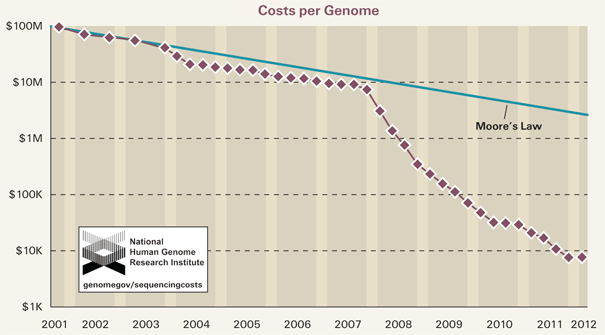
\includegraphics[width=2.5in]{figs/sequencing-costs.png}
  \caption{The cost of genome sequencing has been falling faster than Moore's Law.}
  \label{moore}
\end{figure}
%\end{wrapfigure}

Much of genomic data processing is a statistical inference problem, involving
inferring the DNA sequence of an individual from short ``reads'' of DNA produced
by sequencing machines. Unfortunately, current pipelines take days to execute
for even a single human genome.
%As such, genomic processing is a prime target for scalable inference methods.
To support the processing of thousands to millions of genomes, as well as to
aid in rapid development of new algorithms, we have developed a prototype of the {\bf Big} {\bf G}enomics {\bf I}nference
{\bf E}ngine (BIGGIE), a faster, more scalable, and customizable pipeline for
genomic data processing designed to run on clusters.  

The key insight we propose to exploit is that variation between
genomes of different individuals is non-uniformly distributed, and by
partitioning the genome into regions of high and low complexity, we can apply
different algorithms based on the complexity of each region.
%applying more complex algorithms only to regions of high complexity, we can more efficiently run complex analyses only on regions which are more difficult to analyze.
Abstractly speaking, we \emph{classify} the complexity of a region of the genome
by the quality of read alignments in that region.  Areas with high complexity may
have many poor alignments or alignments with many variations relative to the
reference genome, while areas with low complexity have mostly good and
concordant alignments.
%We may be able to skip regions of very low complexity when performing most analyses, while in areas of high complexity, we may need to perform extra analyses.
Simpler, faster algorithms may be sufficient for processing areas of low
complexity, and therefore we can focus our resources and employ more
sophisticated algorithms on a
much smaller subset of the data. In addition, low-complexity regions give us a
natural location to split the processing of the genome across machines.
This paper explores both of these benefits by showing that simple, fast algorithms
can be effective on a substantial percentage of the genome, and describes how we have 
incorporated them into BIGGIE.

%----------------
\section{Background}
%----------------

DNA sequencing machines analyze cell samples and output data in the form of
\emph{reads}, which are short sequences of DNA.  Variant calling pipelines aim
to convert these raw, noisy short reads into a set of variants that describe
differences between a particular sample and the human reference genome. The
first step in most pipelines involves aligning the reads to an existing human
reference genome.\footnote{An alternative data processing path, which we do not
directly consider in this work, involves \emph{de novo} assembly of the reads
into new genome.} The alignment step is both algorithmically challenging and
computationally intensive, though recent advances have been made, e.g.,
\cite{snap}, and in this work we consider the alignment step as a black-box.

Next, in part based on the alignment from the previous step, variant calling
algorithms are used to identify various types of variants.  Variants can be
categorized as either single-nucleotide polymorphisms (SNPs, pronounced
``snips'') or structural variants.  A SNP is genomic variation in which a
single nucleotide differs from the reference genome.  In contrast, structural
variants are more complex variations relative to the reference genome such as
deletions, duplications, insertions, translocations, etc., and can be as large
as thousands to millions of bases in size.\footnote{`Indels' are a third type
of variant which can roughly be described as a short structural variant, i.e.,
less than 50 nucleotides.} 
%various algorithms are used to call variants   A second tier of analysis includes the detection or ``calling''
%of variants, which consist of differences between individual genomes.  
Once several genomes have been processed with a variant calling pipeline,
subsequent analysis involves population-level inference, including disease gene
mapping, modeling demographic history, and genetic ancestry estimation. Indeed,
this downstream research crucially relies on accurate variant calls from many
individuals.  

However, current variant calling algorithms suffer from both low accuracy and
high computational costs. Variant callers disagree as much as $20\%$ of the
time \cite{haussler}, and it quite difficult, and sometimes not possible, to
run many of the leading structural variant algorithms on full genomes due to
scalability issues \cite{kristalcurtis}.  In this work, we address both the
accuracy and scalability issues associated with leading variant calling tools
and pipelines, and focus on building a general framework for analyzing genome
variation in a distributed fashion.  

All types of human genome variation are of great interest to the bioinformatics
and genetics communities.  Both rare and common SNPs, copy-number differences,
and structural variation have been linked to common diseases, and there is much
ongoing work to entangle the various contributions.  Since SNPs are the most
accessible and easily understood measures of genetic variation, they are also
used to detect admixture, demography, and population structure, in humans and
many other organisms.  Easily obtaining fast and accurate variant calls is thus
very important for downstream biological analysis.
Crucially, we observe that we do not need to perform the same computation on
every base.  Instead, we first learn high and low complexity regions within the
alignment data and subsequently allocate resources accordingly.


%\TODO{Talk more about structural variants}
%SNPs are not the only type of genetic variation; small insertions or deletions
%(indels) in a sequence (with respect to a reference) are common, as well as
%structural variants such as inversions, transpositions, and large-scale indels.
%Copy-number variation (differences in the number of copies of a gene or region
%between individuals) is another common form of variation. 

%\TODO{Talk about significance of the work}
%All types of human genome variation are of great interest to the bioinformatics
%and genetics communities.  Both rare and common SNPs, copy-number differences,
%and structural variation have been linked to common diseases, and there is much
%ongoing work to entangle the various contributions.  Since SNPs are the most
%accessible and easily understood measures of genetic variation, they are also
%used to detect admixture, demography, and population structure, in humans and
%many other organisms.  Easily obtaining fast and accurate variant calls is thus
%very important for downstream biological analysis.

%Moreover, current app and current algorithms, in particular structural variant
%callers  While the current algorithms work well for many of the simpler
%analyses, there is a lack of accurate algorithms involving machine learning and
%population genetics to perform more complex analyses.  In addition, many of the
%existing algorithms are slow, and by improving their performance, we can more
%quickly develop faster and more accurate algorithms.

%\TODO{Instead of focusing just on SNP calling, say that we're building a more general framework}
%More specifically we begin with the problem of calling single-nucleotide
%polymorphisms (SNP, pronounced ``snip''), due to its simplicity compared to
%other types of analyses, yet we plan to design our pipeline with the
%possibility of adding more complex analyses later on.  

%SNP calling is the process of comparing two or more genomes---a reference
%genome, which has been heavily studied and refined, and a set of target
%genomes, which we wish to analyze by comparing to the reference---and returning
%a list of all positions where the two differ by exactly one base.
%SNP calling can additionally refer to the process of comparing several genomes to the reference and returning a list of all single base positions where at least one genome differs from the rest.

%\TODO{Cut down on description of SNP calling}
%The output of this alignment step describes the best alignment position of a read as well as a quantitative alignment error score.
%Sequencing errors in different reads should in theory be independent, although separating errors from SNPs can be challenging in areas of low sequencing coverage (i.e. few aligned reads overlap a given base in the reference).

%--------------
\section{Methods}
%--------------

The following subsections describe the various steps in BIGGIE, explaining what we have implemented and what remains as future work.
%as well as how we plan to build them for an efficient distributed system.  
Several steps
rely on domain knowledge for improved work distribution and communication.
Moreover, the modularity and efficiency of our system will provide a short 
turnaround time between algorithm development and benchmarking, allowing
researchers to quickly explore the design space of different algorithmic
choices and ease of developing new algorithms. Figure~\ref{fig:pipeline} shows our basic pipeline. We assume that we start with an
aligned set of reads for each genome to be processed, in the form of a BAM file
\cite{samtools}.
Sorting the BAM file by the genome index of the alignment is a necessary pre-processing step that can be extremely slow for large datasets, since machines may be limited by amount of memory available.
We do not address sorting here, but leave it as potential future work for improving the pipeline.

\begin{figure}[h!]
  	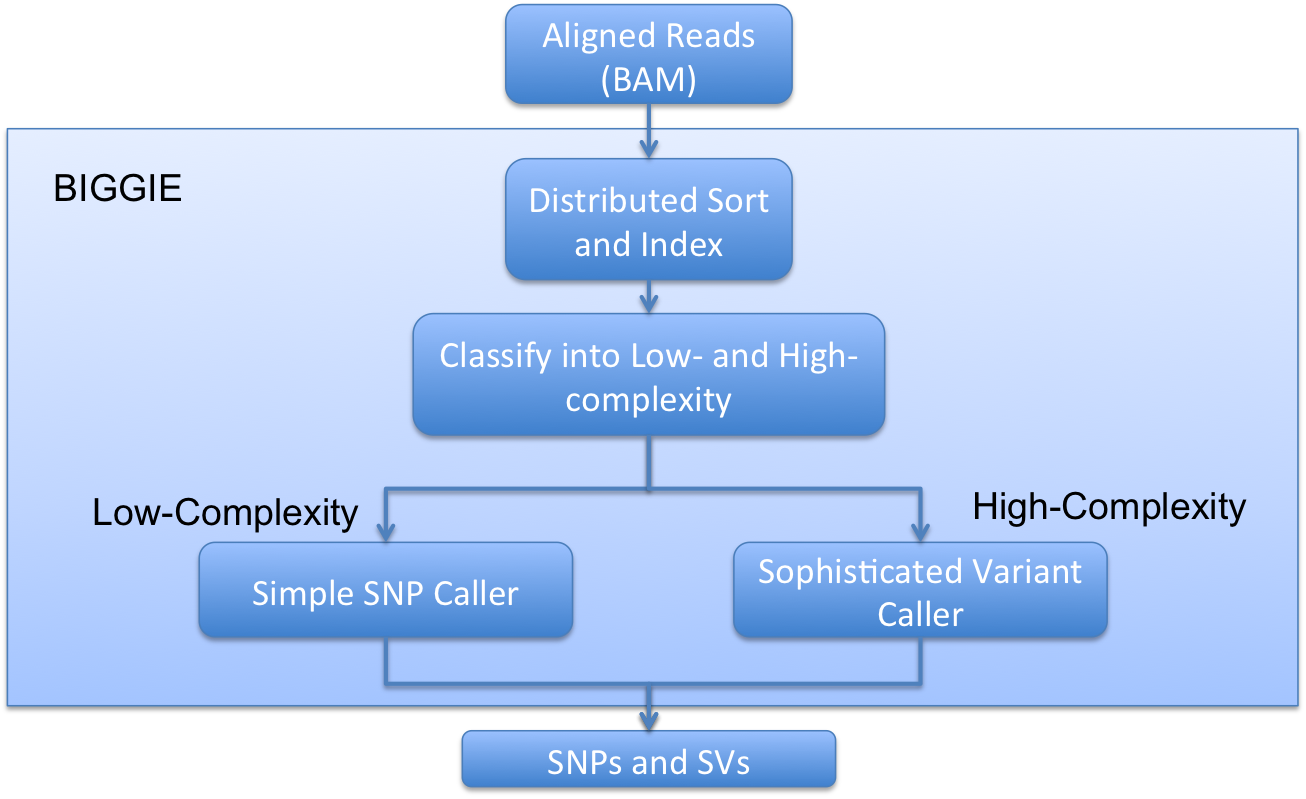
\includegraphics[width=2.6in]{figs/pipeline.png}
	\caption{The BIGGIE pipeline.}
	\label{fig:pipeline}
\end{figure}
 
%% Not related to high/low complexity discussion
%\subsection{BAM Sorting and Indexing}
%The most-common format used for representing an aligned set of reads is the BAM (Binary Sequence Alignment Map) format.
%Most sequence aligners will output a BAM file but the reads are usually randomly ordered.
%For efficiency reasons, most downstream analysis tools require that the reads are sorted by position and that an index file (in BAI format) is generated for fast random access to reads.
%If the reads are not sorted by their alignment position with respect to the reference genome, then variant calling would be very difficult.
%
%Although there already exist several tools which can sort and index BAM files (\cite{bamtools}, \cite{samtools}), they are limited by the amount of memory and may either fail or resort to paging to disk when out of memory.
%To our knowledge there do not exist any distributed BAM file sorters or indexers, and sorting BAM files can be one of the slowest steps of the analysis process.
%Although ideally the BAM file would only be sorted once for each genome, in practice different alignment software (with different parameters) might be used on the same data multiple times.
%We plan to divide up the unsorted BAM file and sort the segments in parallel across a cluster of machines.
%This allows us to keep the BAM files in memory and avoid writing to disk.
%We plan to implement this as a classic merge sort over a cluster.

%----------------------
\subsection{Read Alignment}
%----------------------

The raw reads have been produced by the sequencing platform, the first step in genome analysis is almost always read alignment. This involves mapping the reads to a reference genome, which is often a very computationally challenging problem. BWA \cite{bwa} is a commonly-used short read aligner based on the Burrows-Wheeler transform. SNAP \cite{snap}, is a much faster aligner (developed at Berkeley). Some variant callers have a local realignment step, which is slow but can produce more accurate results. An accurate alignment is key for downstream analysis.

%-------------------------------------
\subsection{Per Base Complexity Classification}
\label{sec:classification}
%-------------------------------------

We first classify each base as either ``high complexity'' or ``low complexity,'' based on the alignment of reads around that base.
This helps us separate the genome into high and low complexity regions later on, which allows us to both operate on different regions in parallel as well as perform different actions based on the quality of the alignments.
Regions of low complexity are characterized by few alignment problems, and regions of high complexity are characterized by either few alignments or many poor alignments.
We can call SNPs relatively easily in
areas of low complexity (see Figure~\ref{low-complexity}(a)), while areas of
high complexity might suggest a structural variant (see
Figure~\ref{low-complexity}(b)).
The intuition is that load-balancing can be improved if we better differentiate between areas of high and low complexity.
Moreover, simpler and faster algorithms can be used to process areas of low complexity, and we can focus our resources and employ more sophisticated algorithms on the high complexity regions.

\begin{figure}[h!]
\begin{center}
\begin{tabular} {@{}c@{}}
  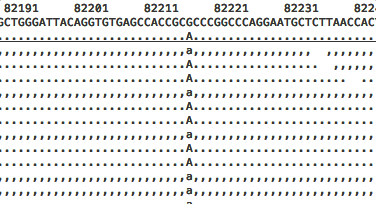
\includegraphics[width=0.40\textwidth]{figs/snp.png} \\ %\qquad\qquad \\
   (a) \\
  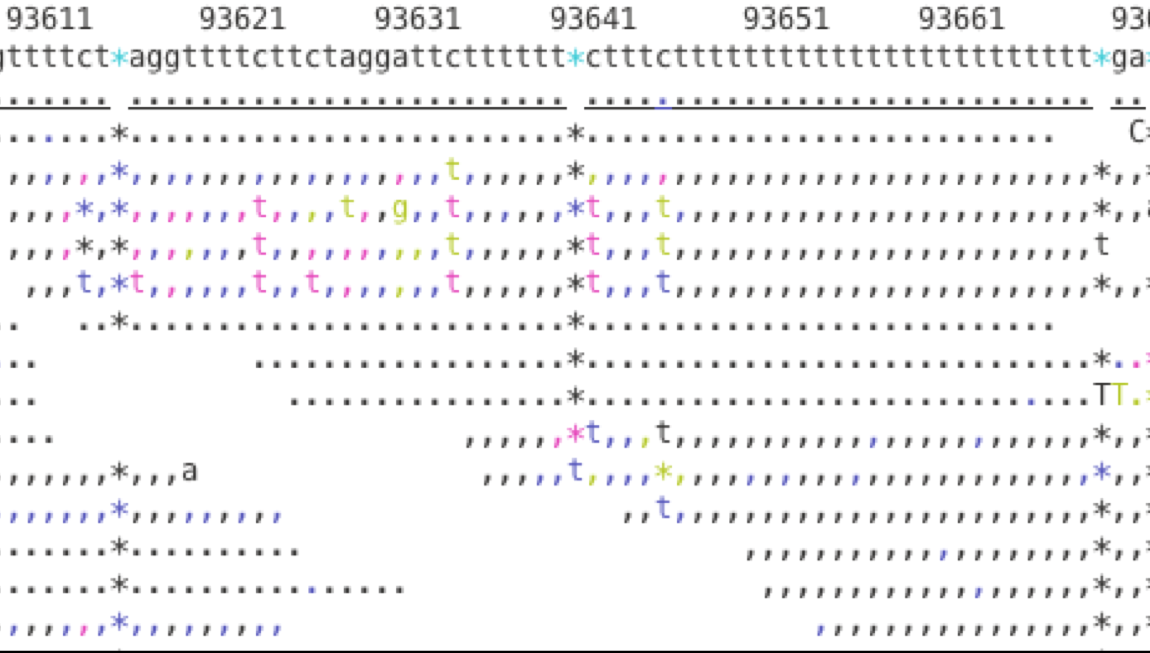
\includegraphics[width=0.40\textwidth]{figs/high-weirdness.png} \\
   (b) \\
\end{tabular}
\end{center}
\caption{(a) \textbf{Low-complexity region} - Samtools alignment viewer on
chromosome 20 of NA12878.  The reference sequence is displayed on top, and base
mismatches are indicated with an actual letter in the read (upper and lower
case letters refer to the strand direction).  In this case, there is an obvious
SNP with the value `A'. (b) \textbf{High-complexity region} - There are many
poor quality alignments with several base mismatches in a relatively small
region. Bases written in displayed in different colors represent varying degrees of poor quality bases. Stars (*) represent a gap in the alignment resulting from an insertion called by at least one read. Many of these poor alignments are due to the highly repetitive
sequence in the area, and more sophisticated techniques, e.g., targeted assembly,
are typically needed to call variants in these regions.  }
  \label{low-complexity}
\end{figure}

%\TODO{what matei has done}
Our goal is to classify bases which match the reference or contain easy-to-call SNPs as low complexity.
Likewise, bases containing harder-to-call SNPs and longer structural variants should be classified as high complexity.
In choosing our heuristics, we consider the following issues with poorly classified bases:
\begin{enumerate}
\item Incorrectly classifying harder-to-call SNPs and structural variants as low complexity will cause us to miss those SNPs and variants because a SNP caller will be unable to find them.
\item Incorrectly classifying simple-to-call SNPs as high complexity will cause us to perform extra work, since they could have been called by a naive SNP caller.
\end{enumerate}

We compute a numerical complexity score for each base as a function of the number of irregularities within a window of 65 bases around the base of interest.
The features we used to calculate our complexity score, along with the relative weights associated with each feature, are described in Table~\ref{complexity}.
Scoring was normalized by the number of aligned reads, and then bases with a score over a threshold of $t_b$ are marked as high-complexity.
We investigate the effects of varying $t$ in the Results section.

Intuitively, we assign a greater weight to insertion and deletion events than substitution and low quality events because the presence of an insertion or deletion suggests that the area around the event may be affected by a misalignment or indel, and therefore a naive SNP caller may not be able to correctly call the variant.
Similarly, unusually low coverage suggests that the reads may have been misaligned to a different area, and unusually high coverage suggests that reads from other areas may have been misaligned to the current area.
Both cases are symptoms of highly repetitive regions (\TODO{citation}).
Lastly, skewed coverage---when more reads of one direction align to the reference than reads of the other direction---is also indicative of misalignments due to systematic biases.
\begin{table}[h!]
\tiny
  \centering
  %\begin{tabular*}{@{\extracolsep{\fill}}|l|l|p{0.7\textwidth}|}
	\begin{tabular}{|l|c|c|}
    \hline Name & Weight & Description \\\hline
    Substitution & 3 & $\#$ aligned reads showing a \\ && substitution with respect to the reference\\\hline
    Insertion & 10 & $\#$ aligned reads showing an \\ && insertion with respect to the reference\\\hline
    Deletion & 10 & $\#$ aligned reads showing a \\ && deletion with respect to the reference\\\hline
    Low Quality & 3 & $\#$ reads aligned with low map quality \\ && (a common indicator of repetitive region)\\\hline
  \end{tabular}
  \caption{Relative weight of features for computing complexity.}
  \label{complexity}
\end{table}

%\TODO{Give estimates on how many high complexity regions there are}

%-----------------------------------
\subsection{Region Compexity Classification}
%-----------------------------------

We then use the complexity scores at each base to define high-complexity regions, which are ranges of bases that may contain both high and low complexity bases.
We build up high-complexity regions in a greedy fashion, adding bases while maintaining that the overall high-complexity base density remains above a threshold $t_r$.
After generating the set of high-complexity regions in this manner, we filter out high-complexity regions that are less than 500 bases long.
We also investigate the effects of changing $t_r$, since increasing $t_r$ may increase the number of truly high-complexity variants which we are unable to call with a simple SNP caller, while decreasing $t_r$ may lower the number of high-complexity regions and improve load balancing.
\TODO{provide more details?}

%-------------------
\subsection{SNP Calling}
%-------------------

\TODO{more details of SNP calling?}
We employ SNP calling on both the low-complexity bases and the low-complexity regions, leaving the task of calling SNPs and structural variants on high-complexity bases and regions for future work.
For these low-complexity bases, our goal is speed and accuracy, which are easier to attain since we are skipping any region we deem complex.
We implemented a simple consensus-based SNP caller, which roughly builds on the intuition that if a SNP exists, then the majority of the reads which cover that position should agree on a common nucleotide which is different from the reference.\footnote{More specifically, we use the standard 80-20 approach \cite{gatk} to deal with diploid genomes and differentiate between homozygous and heterozygous SNPs.}
This algorithm is embarrassingly data-parallel and requires no interprocess communication, and may be trivially parallelized over a cluster, with the only requirement being that the reads need to be distributed once at the beginning.

%\begin{table}
%\small
%	\centering
%	\begin{tabular}{|l|c|c|}
%	\hline 
%	Algorithm & \# false positives & \# false negatives \\
%	\hline 
%	GATK & 66 & 1151 \\
%	\hline
%	Our results & 4 & 3 \\
%	\hline
%	\end{tabular}
%	\caption{Results of SNP calling on simulated reads from Chromosome 20.}
%	\label{SNP-sim}
%\end{table}
%
%\begin{table}
%\small
%	\centering
%	\begin{tabular}{|l|c|c|}
%  \hline
%	Algorithm & \# SNPs & \# Mendelian conflicts  \\
%	\hline
%	CASAVA & 128K & 162 \\
%	\hline
%	Our results & 120K & 84 \\
%  \hline
%	\end{tabular}
%	\caption{Results of SNP calling on Yoruban trio data from Chromosome 20.}
%	\label{SNP-real}
%\end{table}

There are several techniques used for SNP calling,
%. which range from a na\"{i}ve
%consensus-based approach to more complex modeling approaches.  In addition, by
%processing multiple genomes simultaneously, common SNP information can be
%shared between different genomes and be used to provide more accurate SNP
%calls. 
and the modularity of our system allows us to easily switch between these
different options.  More advanced variant detection algorithms exploit common
ancestry among the individuals being studied to pool statistical strength among
samples.  These estimators have been shown to perform better than the na\"{i}ve
approach described above, particularly in the case of missing data and/or low
coverage sequencing experiments \cite{nielsen}.  Accordingly, we plan to design
our system to be flexible enough to support communication between nodes during
this step.  After analyzing several existing SNP callers, such as ones which
create a hidden error model or ones which reuse information across multiple
genomes, we hope to better understand the data dependencies and communication
patterns of common SNP callers.  

%Ideally we would want our system to be interactive -- then the user could run
%one SNP caller, see the output, and run it again in a different way without
%reloading the data into memory.  Reducing the latency between developing an
%algorithm which works on one part of the pipeline and evaluating the results
%will greatly improve the speed and ease of developing new algorithms.  A
%developer will be able to quickly explore the design space of different
%algorithmic choices, which will allow her try more ideas and parameters than in
%existing pipelines.

%------------------------------
\subsection{Structural Variant Calling}
%------------------------------

After processing the low-complexity regions, we are subsequently left with a set
of disjoint high-complexity regions, and we can process 
these regions in an embarrassingly parallel fashion, using more statistically rigorous
and computationally intensive techniques such as targeted assembly \cite{telescoper}.
%In addition to a faster and more accurate SNP caller, we also plan to make our
%pipeline ideal for the development of structural variant calling algorithms.
%Users should be able to run a variant caller on a small subset of the data (as
%identified by the high-complexity metric), obtain fast results, modify and
%iterate, all without needing to redistribute their data.  Current structural
%variant callers are generally slow, inaccurate, and difficult to use.  
Accurate calling of structural variants is a challenging area of bioinformatics
that is not as well-studied as SNP calling, and is hampered by significant
workflow overhead.  By targeting areas in the genome with potential structural
variants and providing a modular platform to develop and test new and existing
algorithms, we hope that our system can foster algorithmic development in this
area.
%These new algorithms are
%likely to require the use of machine learning in order to obtain more accurate
%results.

%\section{Evaluation}
%There are two main types of evaluations we plan to make.
%Since we want to build a faster and more scalable pipeline for SNP calling, we will want to compare our implementation with existing SNP calling pipelines.
%The main data points of interest are performance, memory usage, scalability, and accuracy.
%Measuring accuracy will be the most difficult part of the evaluation, since it is the least standardized metric.
%Our current plan is to compare the SNPs that we call with the SNPs that existing pipelines call as well as existing databases of common SNPs such as dbSNP \cite{dbSNP}.
%
%We also will want to explore the state space of different parameters that we can configure with our pipeline.
%Several of these parameters will include different partitioning schemes, heuristics for determining high- and low-complexity regions, and memory limitations and number of cores.

%-------------------
\section{Implementation}
%-------------------

We implemented Biggie in Scala in about 1000 lines of code, making use of the Picard Java API\TODO{citation} for reading and manipulating BAM and FASTA files.


%---------------
\section{Evaluation}
%---------------

To test the efficacy of our classifier, we used
%real data (Yoruban trio data from the 1000 genomes project \cite{1000genomes}) and 
simulated data from human Chromosome 20. \TODO{cite tvsim} The simulated data consisted of SNPs and other structural variation 
%taken from dbSNP randomly
inserted into the reference for Chromosome 20, which is $63$M bases in length,
of which 94.4\% are known (not Ns).
%Artificial reads were then generated from this simulated genome using simNGS \cite{simNGS}.
We compared BIGGIE to two other variant callers, SAMtools mpileup and GATK (see Section~\ref{sec:relatedWork} for a discussion of these two methods). SAMtools mpileup was run using the best-practices suggestions, with one pass for generating a raw vcf (common variant format) file and one pass for filtering based on quality metrics. GATK was also run using the best-practices suggestions, with one raw vcf pass, a pass for annotating variants (requires training data), and a pass for filtering based on the the annotation step. When running BIGGIE, we evaluated the false negatives only on the low complexity regions, not the high complexity regions where we did not attempt to call variation.

To compare the methods, we only considered SNPs, not more complex structural variation.

%-------------
\section{Results}
%-------------

For the simulated data, 16.6\% of the genome was in a region of high complexity, for $t_r =0.05$. 
%2.2\% of the non-N bases had a
%high complexity score, and for the real data 11.5\% had a high complexity
%score.  The increase for real data is partly due to indels in the reads, but
%probably also due to lower and more variable coverage.  
We hope to further refine this complexity metric and provide the possibility for different types
of classification.  However, this metric already shows that we can drastically
reduce the set of regions we need to analyze in detail.

To verify the
effectiveness of performing SNP calling based on separate high and low
complexity regions, we ran our simple SNP caller only on low-complexity regions.
%using the experimental data described in
%Section~\ref{sec:classification}.  %Even when ignoring high-complexity regions,
%Our SNP caller reports fewer false positives and runs much faster than the
%GATK, an existing tool which can call SNPs ($2$ minutes for our SNP caller
%versus roughly $2$ hours for GATK).  In Table~\ref{SNP-sim}, we compare the
%false positive and false negative rates of GATK with our SNP caller on
%simulated data.  In Table~\ref{SNP-real}, we compare the number of SNPs and
%Mendelian conflicts of CASAVA \cite{casava} with our SNP caller on real data, using the
%Yoruban trio to determine Mendelian conflicts.  

\TODO{discuss the results below}

\begin{figure}[h!]
	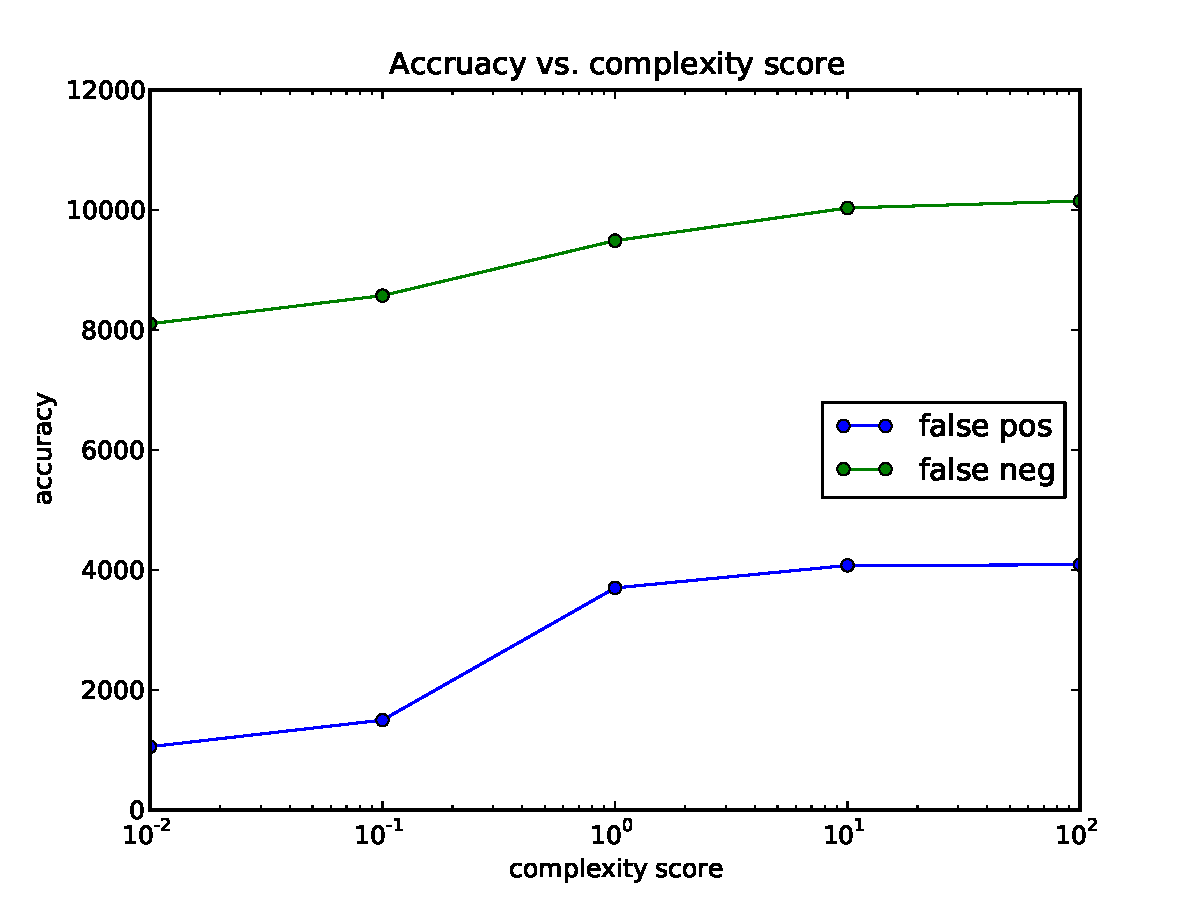
\includegraphics[width=2.7in]{figs/base_accuracy_vs_thresh.pdf}
	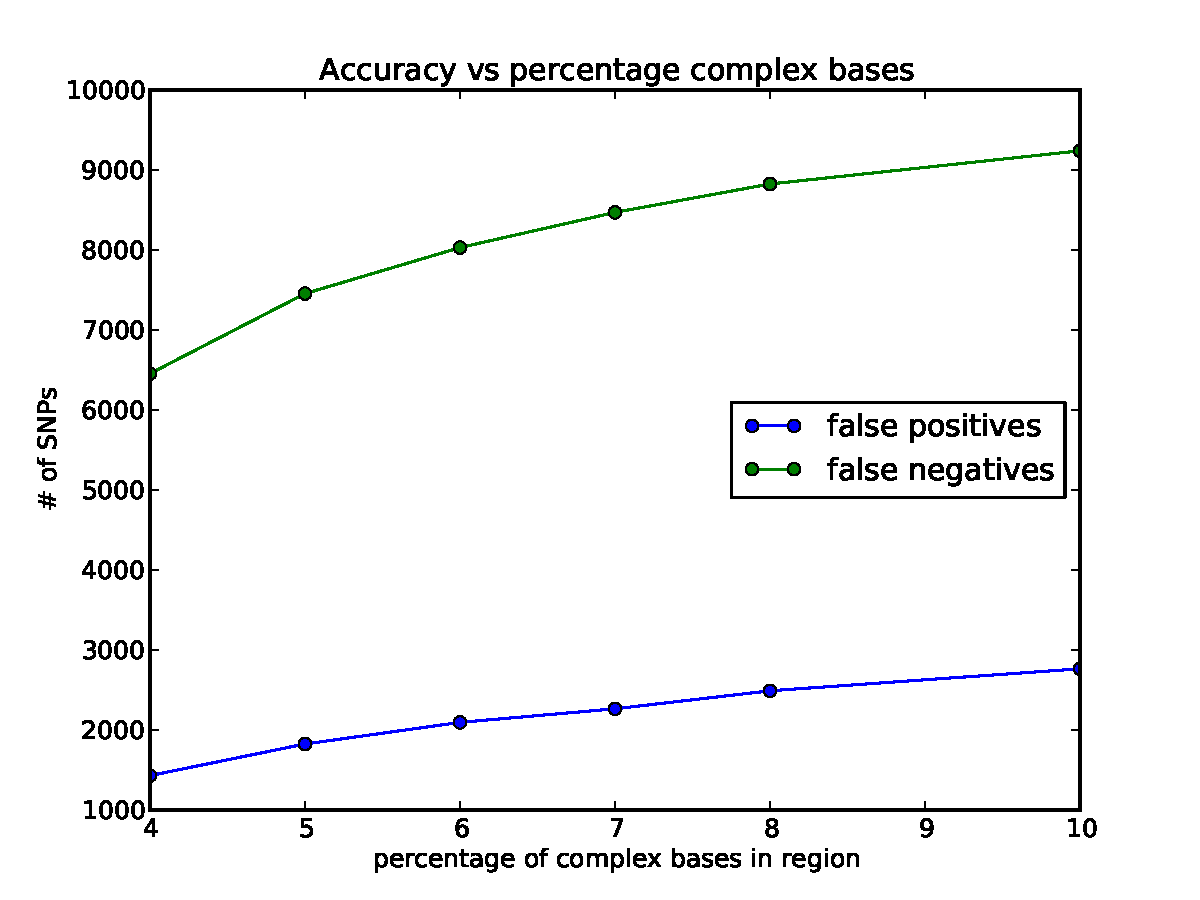
\includegraphics[width=2.7in]{figs/region_accuracy_vs_thresh.pdf}
	\caption{On the left are the per-base results, measuring false negatives only on the regions we called. Both accuracy measures increase as the threshold increases, but the number of correct calls increases as well.  We see a similar pattern on the right for the region results, where the number of false positives and false negatives increase with the density of complex bases in high-complexity regions, but the number of true calls increases as well.}
	\end{figure}

\begin{figure}[h!]
	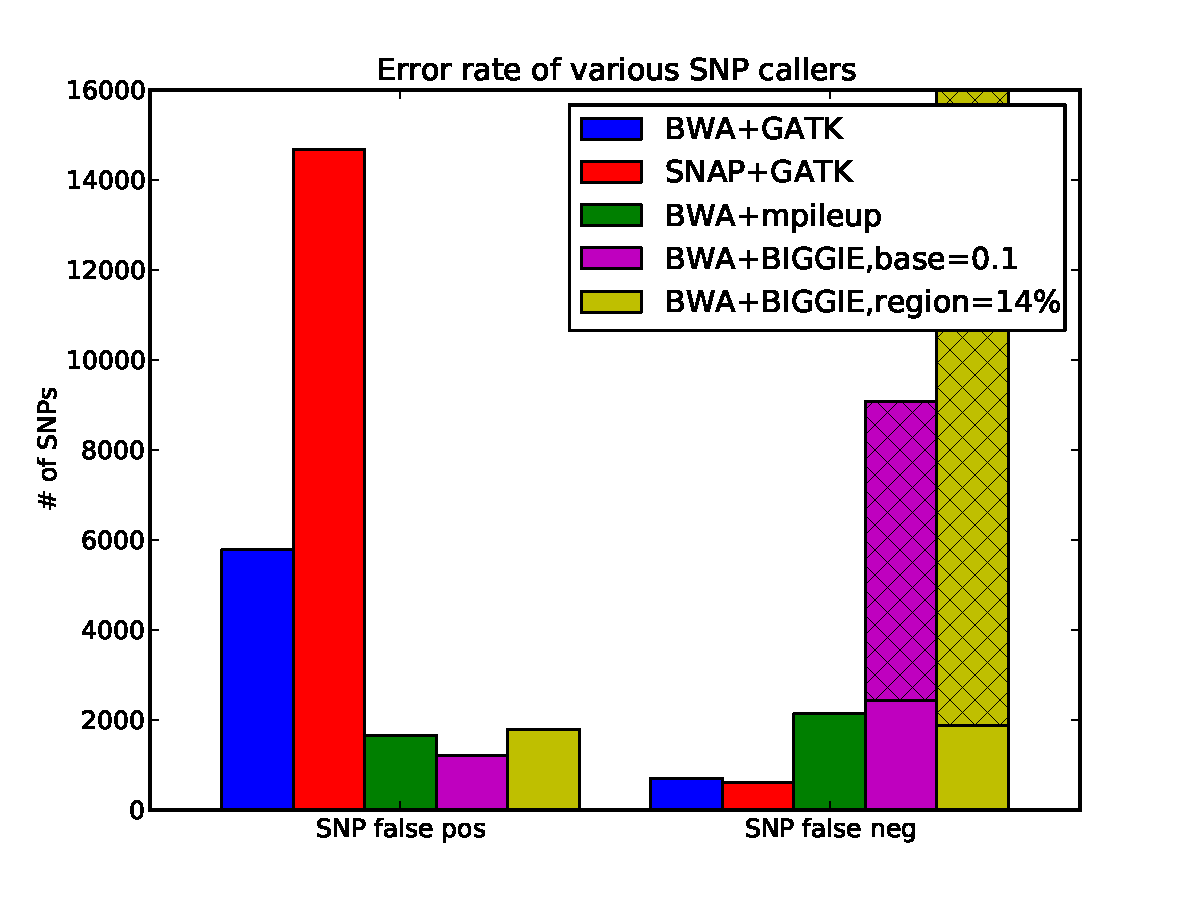
\includegraphics[width=2.7in]{figs/variant_call_results_all.pdf} \hspace{5mm}
	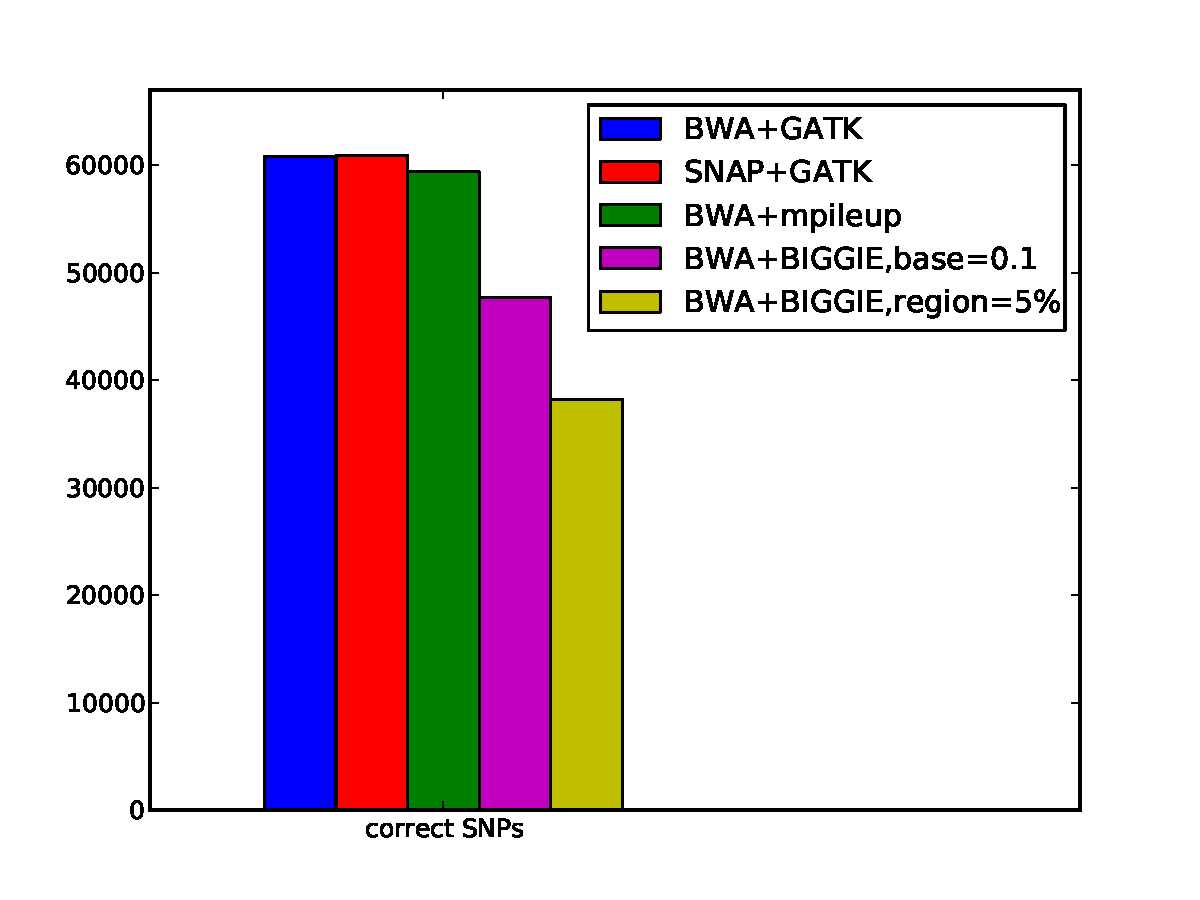
\includegraphics[width=2.7in]{figs/correct_results_all.pdf}
	\caption{Accuracy comparison of BIGGIE with mpileup and GATK. False positives in BIGGIE are often associated with alignment errors or confusion with a small indel. For each algorithm, a very small percentage of correct SNP bases actually have the incorrect (unphased) genotype.} %These numbers using aligner BWA are GATK: 0.48\%, mpileup: 0.25\%, and BIGGIE: 0.35\%}
	\end{figure}


%-----------------
\section{Related Work}
\label{sec:relatedWork}
%-----------------

There are several existing variant callers, such at CASAVA \cite{casava}, SAMtools mpileup \cite{samtools}, GATK \cite{gatk}, and Platypus \cite{platypus}. Each one has unique algorithmic innovations, but there are a core set of steps that are commonly used. CASAVA is Illumina's variant caller, and is not free, so we do not compare against it.

SAMtools mpileup uses a set of alignment filters that attempt to distinguish artifacts from true variation. They also use the concept of a Base Alignment Quality (BAQ), which is the probability that a read base is misaligned. Filtering on BAQ scores helps them elliminate false positive SNPs that are truly small indels. Some drawbacks of mpileup are its slow runtime and somewhat less sophisticated filtering.

%SAMtools is being replaced by GATK as the industry standard.

GATK (Genome Analysis Toolkit) has extensive funtionality beyond variant calling, but has not released the algorithmic details for their current implementation. On a high level, their variant calling algorithm makes a first pass, identifying areas that might be SNPs, indels, or structural variation. Then a second pass requires the user to specify a set of parameters (such as mapping quality, coverage, etc) and a set of outside training data (where the truth is known), so that the algorithm can learn which variants are true and which are noise. The filtered variants are then output. The combination of outside training data and many user-defined parameters makes GATK very difficult to use and understand. Although
GATK does have the ability to perform in a distributed environment, this
functionality is not straightforward for the typical user, and usually GATK
ends up being very slow.  Although GATK provides more functionality than simple
SNP calling, and can be tuned to produce good results, our system is much faster and more
lightweight than GATK.

Most variant callers consider each candidate SNP independently, but the caller
Platypus aggregates information within a window of the genome to take into
account local information. In addition, there are many programs to call more
complex structural variation, although the field is less developed than SNP
calling.  BIGGIE will ideally set us up to efficiently compare structural variant callers later on.

%-----------------------------
\section{Discussion and Future Work}
%-----------------------------

In this project we have demonstrated that we can efficiently identify a simple type of genetic variation (SNPs) by taking advantage of the fact that, for a given individual, some areas will be very complicated, while some will match the reference in straightforward ways. Distinguishing this difference (and hopefully at a finer granularity later on) helps us use our resources well -- simpler algorithms can be used in regions of low complexity, while more sophisticated algorithms can be used in areas of high complexity. Using a simple SNP caller in regions of low complexity (either per base or by region), we obtain good variant calls, with a very low number of false positives, which was our goal. 
\TODO{discuss false negatives when we know more}

There are many interesting areas of future work, and we plan for implementation to continue on BIGGIE. The main areas include scaling up to the entire genome and taking appropriate memory and distribution decisions as difficulties arise, as well as better definitions for what makes a base or a region highly complex. Finally, we would like to make BIGGIE an environment where structural variant callers can be run and compared without reloading data into memory.  Having an end-to-end pipeline will help us learn how mistakes early on can lead to downstream errors, so we can make corrections efficiently. 

%\end{multicols}
\onecolumn

%\section{References}
\newpage
\begin{thebibliography}{1}

\bibitem{telescoper} Bresler M., Sheehan S., Chan A., and Song, Y., ``Telescoper: {\it de novo} assembly of highly repetitive regions.'' {\em Bioinformatics} (2012), 28: 311-317.

\bibitem{bamtools} Barnett D., Garrison E., Quinlan A., Str\"{o}mber M., and Marth G., ``BamTools: a C++ API and toolkit for analyzing and managing BAM files.'' {\em Bioinformatics} (2011), 27: 1691-1692.

\bibitem{gatk} DePristo M., Banks E., Poplin R., Garimella K., Maguire J., Hartl C., Philippakis A., del Angel G., Rivas M., Hanna M., McKenna A., Fennell T., Kernytsky A., Sivachenko A., Cibulskis K., Gabriel S., Altshuler D., and Daly M., ``A framework for variation discovery and genotyping using next-generation DNA sequencing data.'' {\em Nature Genetics} (2011), 43:491-498.

\bibitem{haussler} Haussler D. Keynote Address: The UCSC Cancer Genomics Hub. (2012) https://www.usenix.org/conference/osdi12/keynote-address.

\bibitem{samtools} Li H., Handsaker B., Wysoker A., Fennell T., Ruan J., Homer N., Marth G., Abecasis G., Durbin R. and 1000 Genome Project Data Processing Subgroup, ``The Sequence alignment/map (SAM) format and SAMtools.'' {\em Bioinformatics} (2009), 25: 2078-9.

\bibitem{bwa} Li H. and Durbin R. ``Fast and accurate short read alignment with Burrows-Wheeler Transform.'' {\em Bioinformatics} (2009), 25:1754-60.

\bibitem{dbSNP} National Center for Biotechnology Information (US), (2005-), http://www.ncbi.nlm.nih.gov/projects/SNP/.

\bibitem{nielsen} Nielsen, R., Paul, J.S., Albrechtsen, A., and Song, Y.S. ``Genotype and SNP calling from next-generation sequencing data.'' {\em Nature Reviews Genetics} (2011), 12:443-451. 

\bibitem{platypus} Rimmer A., Mathieson I., Lunter G., and McVean G., ``Platypus: An Integrated Variant Caller'' (2012), www.well.ox.ac.uk/platypus.

\bibitem{kristalcurtis} Curtis, K., personal communication, (2012).

\bibitem{schuster} Schuster, S. ``Next-generation sequencing transforms today's biology.'' {\em Nature Methods} (2008), 5: 16-18.

\bibitem{1000genomes} The 1000 Genomes Project Consortium. ``A map of human genome variation from population-scale sequencing.'' {\em Nature} (2010) 467:1061–1073.

\bibitem{snap} Zaharia M., Bolosky W., Curtis K., Fox A., Patterson P., Shenker S., Stoica I., Karp R., Sittler T., ``Faster and More Accurate Sequence Alignment with SNAP.'' (2011) http://arxiv.org/abs/1111.5572.

\bibitem{simNGS} Massingham T. simNGS and simLibrary -- Software for Simulating Next-Gen Sequencing Data. (2010) http://www.ebi.ac.uk/goldman-srv/simNGS/.

\bibitem{casava} CASAVA. (2012) http://support.illumina.com/sequencing/sequencing\_software/casava.ilmn.
\end{thebibliography}

\end{document}
